%!TEX root = ../main.tex



\section{Εισαγωγή}

\lettrine[findent=2pt]{\fbox{\textbf{Η}}}{} ρύθμιση του PID ελεγκτή έχει να κάνει με την απόδοση τιμών στο συντελεστή κάθε όρου, έτσι ώστε καθένας από αυτούς να επηρεάσει θετικά την απόκριση του συστήματος, ενώ ταυτόχρονα να μετριαστούν όσο γίνεται περισσότερο τα αρνητικά του κάθε όρου. Ο τύπος της διεργασίας επηρεάζει το τι είναι επιθυμητό από τον έλεγχό της. Για παράδειγμα, κάποιες διεργασίες μπορεί να μην ανέχονται υπέρβαση (\emph{overshoot}) της απόκρισής τους και αυτό να θέτει και περιορισμούς στο χρόνο ανύψωσης (\emph{rise time}). Αντιθέτως, άλλες διεργασίες μπορεί να παρουσιάζουν ανοχή σε ένα ποσοστό υπέρβασης και έτσι να επιτρέπουν να αυξηθεί ο χρόνος ανύψωσης.

Παρόλο που η υλοποίηση του PID ελεγκτή είναι σχετικά ευθύς και απλή διαδικασία, η σωστή ρύθμισή του είναι πιο περίπλοκο ζήτημα. Αυτό συμβαίνει επειδή απαιτεί κατανόηση του τρόπου με τον οποίο κάθε όρους του PID επηρεάζει τη συνολική απόκριση. Ένας κακώς ρυθμισμένος PID ελεγκτής θα εμφανίσει αρκετά προβλήματα απόδοσης όπως: ταλαντώσεις, μη επαρκή απόσβεση, υπέρβαση, αργούς χρόνους ανόδου ή καθόδου και άλλα. Σε αυτό το κεφάλαιο θα γίνει μια περιγραφή κάποιων διαδεδομένων τεχνικών ρύθμισης που συναντάει κανείς στη βιβλιογραφία (υπάρχουν πολλές πιο εξελιγμένες μέθοδοι ρύθμισης αλλά υπόκεινται σε εμπορικές πατέντες) καθώς και των προβλημάτων που οφείλονται σε κακή ρύθμιση του PID ελεγκτή.

Η ανάλυση των τεχνικών ρύθμισης θα γίνει με αναφορά στα κέρδη $K_p$, $K_i$ και $K_d$, δηλαδή θα αφορά την παράλληλη μορφή του PID ελεγκτή της Εξίσωσης (\ref{eq:parallel_pid}) και όχι την τυποποιημένη μορφή της Εξίσωσης (\ref{eq:standard_pid}), παρόλο που η δεύτερη χρησιμοποιήθηκε στην εργασία αυτή. Αυτό συμβαίνει γιατί ο αναγνώστης είναι πιο εύκολο να καταλάβει πώς επηρεάζουν τα κέρδη την απόκριση του συστήματος χρησιμοποιώντας την πρώτη εξίσωση. Φυσικά, οι ίδιοι κανόνες ισχύουν και για τις παραμέτρους $T_i$ και $T_d$ της τυποποιημένης μορφής, έχοντας πάντα υπόψιν τις εξισώσεις που συνδέουν τις παραμέτρους των δύο αυτών σχέσεων.

\section{Τεχνικές ρύθμισης}

\subsection{Χειροκίνητη ρύθμιση}

Η πρώτη και πιο φυσική μέθοδος είναι η χειροκίνητη ρύθμιση του ελεγκτή από έναν χειριστή. Σε αυτή τη μέθοδο αρχικά τα κέρδη $K_i$ και $K_d$ ισούνται με το μηδέν. Στη συνέχεια, αυξάνουμε το αναλογικό κέρδος $K_p$ μέχρι το σύστημα να αρχίσει να ταλαντώνεται ελαφρώς και ο χρόνος ανύψωσης να είναι ικανοποιητικός. Έπειτα, αυξάνουμε το ολοκληρωτικό κέρδος $K_i$ έως ότου να εξαλειφθεί το σφάλμα μόνιμης κατάστασης, σε λογικό χρόνο για τη συγκεκριμένη διεργασία. Σε αυτό το σημείο πρέπει να έχουμε στο μυαλό μας ότι μεγαλύτερο ολοκληρωτικό κέρδος σημαίνει και μεγαλύτερη αστάθεια του συστήματος. Τέλος, αν χρειάζεται, αυξάνουμε το κέρδος παραγώγου $K_d$ για να βελτιώσουμε τη σταθερότητα του συστήματος καθώς και την απόκρισή του σε αλλαγή φορτίου ή σε κάποια διαταραχή. Εδώ πρέπει να έχουμε υπόψη μας ότι μεγάλο κέρδος παραγώγου θα προκαλέσει υπερβολική ανταπόκριση σε μεταβολές και υπέρβαση.

Ένας βρόχος PID που έχει ρυθμιστεί για να επιτύχει μια γρήγορη απόκριση συνήθως θα υπερβεί ελαφρώς την επιθυμητή τιμή ως συνέπεια της γρήγορης ``ρύθμισης" του. Εντούτοις, μερικά συστήματα δεν μπορούν να ανεχθούν οποιαδήποτε υπέρβαση, οπότε στην περίπτωση αυτή απαιτείται σύστημα κλειστού βρόχου, το οποίο θα πρέπει να έχει μικρότερο αναλογικό κέρδος $K_p$ από αυτό ενός συστήματος που μπορεί να ανεχτεί κάποιο ποσοστό υπέρβασης. Στον Πίνακα \ref{table:parameters} φαίνεται πώς ο κάθε όρος του ελεγκτή επηρεάζει την απόκριση του συστήματος υπό έλεγχο.

\begin{table}[H]
\begin{center}
\begin{tabular}{ |c|c|c|c|c|c| }
\hline
\thead{Παράμετρος} & \thead{Χρόνος \\ ανύψωσης} & \thead{Υπέρβαση} & \thead{Μόνιμο \\ σφάλμα} & \thead{Χρόνος \\ ηρεμίας} & \thead{Ευστάθεια}\\ \hline
\thead{$K_p$} & \thead{Μείωση} & \thead{Αύξηση} & \thead{Μείωση} & \thead{Μικρή \\ αλλαγή} & \thead{Χειροτέρευση} \\ \hline
\thead{$K_i$} & \thead{Μείωση} & \thead{Αύξηση} & \thead{Εξάλειψη} & \thead{Αύξηση} & \thead{Χειροτέρευση} \\ \hline
\thead{$K_d$} & \thead{Μικρή \\ αλλαγή} & \thead{Μείωση} & \thead{Καμία \\ αλλαγή} & \thead{Μείωση} & \thead{Βελτίωση} \\
\hline
\end{tabular}
\caption{Επίδραση στο σύστημα, της αύξησης κάθε παραμέτρου ανεξάρτητα από τις άλλες}
\label{table:parameters}
\end{center}
\end{table}

\subsection{Μέθοδος Ziegler–Nichols}

Ίσως η πιο γνωστή μέθοδος ρύθμισης ενός PID ελεγκτή είναι η \emph{Ziegler-Nichols}. Η μέθοδος αυτή έχει πάρει το όνομά της από τους \emph{John G. Ziegler} και \emph{Nathaniel B. Nichols} που την παρουσίασαν το $1942$ και χρησιμοποιείται ακόμα και σήμερα. Όπως και στην προηγούμενη μέθοδο, στην αρχή τα κέρδη $K_i$ και $K_d$ τίθενται ίσα με το μηδέν. Στη συνέχεια αυξάνουμε το κέρδος $K_p$ μέχρι το σύστημα αυξάνεται μέχρι την τιμή που θα οδηγήσει το σύστημα να εκτελεί ταλαντώσεις σταθερού πλάτους και σταθερής περιόδου. Η τιμή αυτή του κέρδους ονομάζεται απόλυτο κέρδος, $\boldsymbol{K_u}$, και η περίοδος των ταλαντώσεων ονομάζεται απόλυτη περίοδος, $\boldsymbol{T_u}$. Αυτές τις δύο παραμέτρους τις χρησιμοποιούμε για να ορίσουμε τα κέρδη όπως φαίνεται στον Πίνακα \ref{table:zn_method}. Στον πίνακα αυτόν έχουν υπολογιστεί οι παράμετροι $T_i$ και $T_d$ της τυποποιημένης μορφής του PID αλγορίθμου \cite{ziegler-nichols}. Αυτό έγινε επειδή αυτή η μορφή των παραμέτρων θα χρησιμοποιηθεί αργότερα για την αυτόματη ρύθμιση του ελεγκτή της εργασίας.


\begin{table}[H]
 \begin{center}
 \begin{tabular}{|c|c|c|c|}
 \hline
 Τύπος ελέγχου & $K_p$ & $T_i$ & $T_d$ \\ \hline
 P & $0.50K_u$ & -- & -- \\ \hline
 PI & $0.45K_u$ & $T_u/1.2$ & -- \\ \hline
 PD & $0.80K_u$ & -- & $T_u/8$ \\ \hline
 PID & $0.60K_u$ & $T_u/2$ & $T_u/8$ \\ \hline
 \end{tabular}
 \caption{Παράμετροι Ziegler-Nichols ανάλογα τον τύπο του ελεγκτή}
 \label{table:zn_method}
 \end{center}
\end{table}

Οι κανόνες ρύθμισης Ziegler-Nichols, συνήθως οδηγούν σε συστήματα με ιδιαίτερα υψηλή υπέρβαση και ``επιθετική" (``aggressive") απόκριση. Δεν παρέχουν δηλαδή μια έτοιμη λύση ρύθμισης αλλά τις περισσότερες φορές προσφέρουν ένα αρκετά ικανοποιητικό σημείο εκκίνησης από το οποίο ο χειριστής μπορεί να ξεκινήσει να τροποποιεί τα κέρδη έτσι ώστε να έχει την επιθυμητή απόκριση.

\subsection{Μέθοδος Tyreus-Luyben}

Μια μέθοδος πολύ παρόμοια με τη μέθοδο Ziegler-Nichols που περιγράφηκε πριν είναι η μέθοδος Tyreus-Luyben. Και αυτή βασίζεται στην απόλυτη συχνότητα (\emph{$T_u$}) και στο απόλυτο κέρδος (\emph{$K_u$}) του συστήματος. Το μόνο που αλλάζει σε σχέση με την προηγούμενη μέθοδο είναι οι τιμές των κερδών ανάλογα με τον τύπο ελέγχου. Οι τιμές αυτές φαίνονται στον Πίνακα \ref{table:tl_method}.

\begin{table}[H]
 \begin{center}
 \begin{tabular}{|c|c|c|c|}
 \hline
 Τύπος ελέγχου & $K_p$ & $T_i$ & $T_d$ \\ \hline
% P & $0.50K_u$ & - & - \\ \hline
 PI & $K_u/3.2$ & $2.2T_u$ & -- \\ \hline
% PD & $0.80K_u$ & - & $T_u/8$ \\ \hline
 PID & $K_u/2.2$ & $2.2T_u$ & $T_u/6.3$ \\ \hline
 \end{tabular}
 \caption{Παράμετροι Tyreus-Luyben ανάλογα τον τύπο του ελεγκτή}
 \label{table:tl_method}
 \end{center}
\end{table}

\subsection{Μέθοδος Cohen-Coon}

Αυτή η μέθοδος αναπτύχθηκε το $1953$ και βασίζεται σε ένα μοντέλο συστήματος πρώτης τάξης με μία χρονοκαθυστέρηση. Παρόμοια με τη μέθοδο Ziegler-Nichols, η μέθοδος αυτή προτείνει ένα σύνολο παραμέτρων συντονισμού για να δώσει μια απόκριση κλειστού βρόχου με λόγο απόσβεσης $1/4$. Σε αντίθεση όμως με τις δύο προηγούμενες μεθόδους που χρησιμοποιούν στοιχεία της απόκρισης συχνότητας του συστήματος για να βγάλουν υπολογίσουν τα κέρδη του ελεγκτή, αυτή η χρησιμοποιεί στοιχεία από την βηματική απόκριση (\emph{Step response}) του συστήματος.

\subsection{Άλλες μέθοδοι και περαιτέρω πληροφορίες}

Στην ενότητα αυτή περιγράφηκαν οι πιο γνωστές και διαδεδομένες τεχνικές ρύθμισης ενός PID ελεγκτή. Βέβαια τα πολλά χρόνια εφαρμογής των PID ελεγκτών στη βιομηχανία, καθώς και η ανάγκη για όλο και πιο λεπτομερή και στιβαρό έλεγχο έχουν οδηγήσει στην ανάπτυξη πολλών ακόμα μεθόδων και τεχνικών. Βέβαια πολλές από αυτές προστατεύονται από νόμους περί πνευματικής ιδιοκτησίας. Εδώ αναλύθηκαν μόνο οι μέθοδοι που χρησιμοποιήθηκαν στο πρακτικό κομμάτι της εργασίας. Κάποιος που ενδιαφέρεται για μια αναλυτική προσέγγιση σε πολλές μεθόδους ρύθμισης καθώς και να μάθει για τα πλεονεκτήματα και τους περιορισμούς της κάθε μίας μπορεί να ανατρέξει στις πηγές \cite{astrom}, \cite{yun}, \cite{kristian}.

\section{Περιορισμοί και προβλήματα κακής ρύθμισης}

\lettrine[findent=2pt]{\fbox{\textbf{Π}}}{αρόλο} που οι ελεγκτές PID είναι εφαρμόσιμοι σε πολλά προβλήματα ελέγχου και συχνά παρέχουν ικανοποιητικό έλεγχο χωρίς βελτιώσεις ακόμα και όταν έχουν ρυθμιστεί ``στο περίπου", μπορούν να έχουν χαμηλή απόδοση σε ορισμένες εφαρμογές και σχεδόν ποτέ δεν παρέχουν βέλτιστο έλεγχο. Η βασική δυσκολία με τον έλεγχο PID είναι ότι είναι ένα σύστημα ελέγχου ανατροφοδότησης, με σταθερές παραμέτρους και χωρίς άμεση γνώση της διαδικασίας και έτσι η συνολική απόδοση είναι αντιδραστική και συμβιβαστική.

Οι ελεγκτές PID, όταν χρησιμοποιούνται μόνοι τους, μπορούν να έχουν χαμηλή απόδοση όταν τα κέρδη τους πρέπει να μειωθούν, έτσι ώστε το σύστημα ελέγχου να μην παρουσιάζει υπέρβαση, να μην ταλαντώνεται ή να μην κυνηγάει την τιμή ρύθμισης του ελέγχου. Παρουσιάζουν επίσης προβλήματα όταν εμφανίζονται μη γραμμικότητες, μπορεί να ανταλλάσουν την πιο ομαλή απόκριση έναντι του χρόνου απόκρισης, να μην αντιδρούν στην αλλαγή της συμπεριφοράς της διαδικασίας (ας πούμε, η διαδικασία αλλάζει μετά από το ζέσταμα) και να έχουν καθυστέρηση στην αντιμετώπιση μεγάλων διαταραχών.

\subsection{Γραμμικότητα}

Ο PID ελεγκτής είναι ένα γραμμικό και ιδιαίτερα συμμετρικό σύστημα. Συνεπώς, η απόκρισή του όταν εφαρμόζεται σε ένα μη γραμμικό σύστημα είναι μεταβλητή. Για παράδειγμα, στον έλεγχο της θερμοκρασίας, μια κοινή περίπτωση χρήσης είναι η ενεργή θέρμανση (μέσω θερμαντικού στοιχείου), αλλά η παθητική ψύξη (θέρμανση χωρίς ψύξη), οπότε η υπέρβαση που μπορεί να προκαλεί ο ελεγκτής διορθώνεται αργά - δεν μπορεί να εξαναγκαστεί προς τα κάτω. Σε αυτή την περίπτωση ο PID θα πρέπει να ρυθμιστεί ώστε να παρέχει υπεραποσβενούμενη απόκριση, για να αποτρέψει ή να μειώσει την υπέρβαση, αν και αυτό μειώνει την απόδοση του συστήματος (αυξάνει το χρόνο ηρεμίας).

\subsection{Θόρυβος στον παράγωγο όρο}

Ένα πρόβλημα με τον παράγωγο όρο είναι ότι ενισχύει τη μέτρηση υψηλής συχνότητας ή το θόρυβο της διαδικασίας, με αποτέλεσμα να προκαλούνται μεγάλες αλλαγές στην έξοδο. Συχνά είναι χρήσιμο να φιλτράρονται οι μετρήσεις με φίλτρο χαμηλής διέλευσης (\emph{low-pass filter}) για να αφαιρείται ο θόρυβος υψηλής συχνότητας. Καθώς το φιλτράρισμα χαμηλής διέλευσης και ο παράγωγος έλεγχος μπορούν να ακυρώνουν ο ένας στον άλλο, η ποσότητα φιλτραρίσματος είναι περιορισμένη. Μπορεί επίσης να χρησιμοποιηθεί ένα μη γραμμικό διάμεσο φίλτρο, το οποίο βελτιώνει την αποδοτικότητα φιλτραρίσματος και την πρακτική απόδοση \cite{chong}. Σε ορισμένες περιπτώσεις, ο παράγωγος όρος μπορεί να απενεργοποιηθεί με λίγες διαφοροποιήσεις στη συνολική απόδοση.

\subsection{Ταλαντώσεις}

Η ταλάντωση είναι ένα από τα πιο περίπλοκα ζητήματα επίδοσης στους PID ελεγκτές και μπορεί να είναι αποτέλεσμα πολλών παραγόντων. Η πιο συνηθισμένη αιτία είναι το πολύ μεγάλο αναλογικό κέρδος (Σχήμα \ref{fig:proportional_oscillation}). Μια δεύτερη αιτία είναι ένας ελεγκτής που βασίζεται κυρίως στον ολοκληρωτικό του όρο (Σχήμα \ref{fig:integral_oscillations}) επειδή το σφάλμα που έχει συσσωρευτεί ενώ η μετρούμενη μεταβλητή είναι κάτω από το καθορισμένο σημείο χρειάζεται χρόνο για να διορθωθεί ενώ η μετρούμενη μεταβλητή είναι πάνω από το καθορισμένο σημείο. Ο ολοκληρωτικός όρος στη συνέχεια αρχίζει να συσσωρεύει σφάλμα στην αντίθετη κατεύθυνση, το οποίο δεν θα διορθωθεί μέχρις ότου η μετρούμενη μεταβλητή να διασχίσει ξανά το καθορισμένο σημείο. Σε αυτή την περίπτωση ο αναλογικός όρος ενεργεί ως αποσβεστήρας. Τρίτον, κάτι που εύκολα παραβλέπεται πολλές φορές, είναι ότι το το φυσικό σύστημα που ελέγχεται θα μπορούσε να έχει από μόνο του ταλαντευόμενο χαρακτήρα και συνεπώς η ύπαρξη ταλαντώσεων στο σύστημα ίσως είναι αποδεκτή. Αυτό δεν σημαίνει απαραίτητα κακή ρύθμιση του PID ελεγκτή.

\begin{figure}[h]
  \centering
  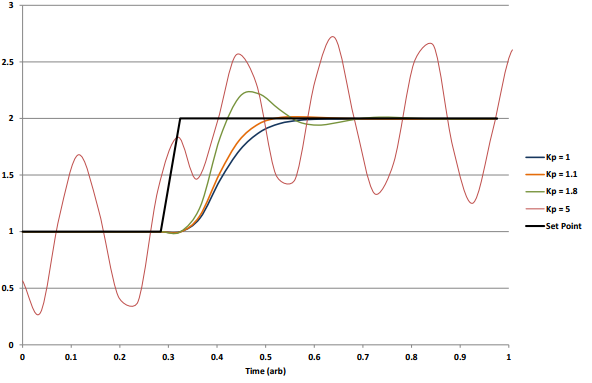
\includegraphics[width=\textwidth]{proportional_oscillation}
  \caption{Απόκριση της μετρούμενης μεταβλητής στην αύξηση του αναλογικού κέρδους}
  \label{fig:proportional_oscillation}
\end{figure}

\begin{figure}[h]
  \centering
  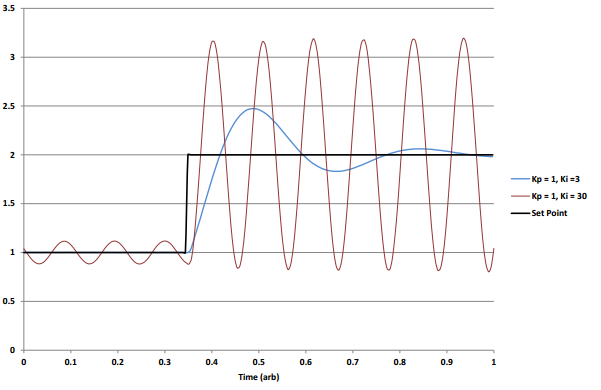
\includegraphics[width=\textwidth]{integral_oscillations}
  \caption{Ταλαντώσεις λόγω υψηλού ολοκληρωτικού κέρδους}
  \label{fig:integral_oscillations}
\end{figure}

Η συχνότητα του ελεγκτή είναι ο ρυθμός με τον οποίο ο βρόχος ελέγχου λειτουργεί και η έξοδος τροφοδοσίας ενημερώνεται μία φορά ανά κύκλο. Αυτή η συμπεριφορά απλής ενημέρωσης μπορεί να είναι προβληματική αν το αναλογικό κέρδος είναι υπερβολικά υψηλό. Ένα μικρό σφάλμα παράγει μια μεγάλη έξοδο, η οποία προκαλεί μεγάλη μεταβολή στη μετρούμενη μεταβλητή, ακόμη και σε έναν κύκλο. Εάν η αλλαγή αυτή μεταβάλλει τη μετρούμενη μεταβλητή πέρα από το καθορισμένο σημείο, τότε η έξοδος αντιστρέφει την πολικότητα για τον επόμενο κύκλο. Αν η μετρούμενη μεταβλητή συνεχίζει να πηδάει από το κύκλο σε κύκλο, τότε ο ελεγκτής ταλαντώνεται. Αν το κέρδος είναι αρκετά υψηλό και προκαλεί την μεταπήδηση της μετρούμενης μεταβλητής με αυξανόμενο μέγεθος σφάλματος, τότε ο ελεγκτής θεωρείται ασταθής. Η πιο γρήγορη λύση είναι η μείωση του αναλογικού κέρδος. Ωστόσο, η αύξηση της συχνότητας του ελεγκτή, αν αυτό είναι δυνατόν, θα βοηθήσει επίσης.

Αυτός είναι εγγενής περιορισμός ενός ψηφιακού ελεγκτή. Θα υπάρχει πάντα ταλάντωση σε κάποιο βαθμό. Εκτός από το ζήτημα συχνότητας βρόχου που έχει ήδη περιγραφεί, η έξοδος της τροφοδοσίας μπορεί να μειωθεί μόνο σε κάποια πεπερασμένη τιμή και τίποτα μικρότερο. Το πρόβλημα τότε γίνεται ζήτημα πόσο μπορεί να μειωθεί η ταλάντωση. Ένας απόλυτα συνεχής ελεγκτής δεν έχει αυτό το πρόβλημα επειδή η έξοδος συνεχώς ενημερώνεται μαζί με το μεταβαλλόμενο σφάλμα. Ωστόσο, η ταλάντωση από τους περιορισμούς συχνότητας εξακολουθεί να συμβαίνει στον συνεχή έλεγχο PID. Αυτοί οι ελεγκτές είναι αναλογικά κυκλώματα και εξακολουθούν να έχουν μια αποτελεσματική συχνότητα λειτουργίας που προκύπτει από αντιδραστικά στοιχεία που προκαλούν χρονική υστέρηση μεταξύ της εξόδου και της εισόδου.

Η ταλάντωση λόγω ενός υψηλού ολοκληρωτικού κέρδους μπορεί να μειωθεί είτε μειώνοντας το ολοκληρωτικό κέρδος (προφανής λύση) είτε αυξάνοντας το αναλογικό κέρδος (όχι άμεσα προφανές). Η αναλογική δράση θα επιβραδύνει τις ταλαντώσεις που προκαλούνται από την ολοκληρωτική δράση. Αυτό το παράδειγμα παρουσιάζει τη δυσκολία συντονισμού του PID ελεγκτή. Ο χρήστης πρέπει να αποφασίσει ποια χαρακτηριστικά των αποκρίσεων του ελεγκτή είναι απαραίτητα, επιθυμητά και ποια είναι μη αποδεκτά. Κάθε όρος έχει υπέρ και κατά και πρέπει να καθοριστεί η προτεραιότητα των χαρακτηριστικών του ελεγκτή πριν από την προσπάθεια ρύθμισης του συστήματος.

\subsection{Χρόνος ανόδου και Υπέρβαση}

Ο χρόνος ανόδου της μετρούμενης μεταβλητής είναι ο χρόνος που απαιτείται για την μετρούμενη μεταβλητή να φτάσει στο καθορισμένο σημείο μετά από μια αλλαγή. Ένας γρήγορος χρόνος ανόδου είναι επιθυμητός για προφανείς λόγους, αλλά ένας πολύ μικρός χρόνος ανόδου θα προκαλέσει υπέρβαση της μετρούμενης μεταβλητής από το καθορισμένο σημείο. Η υπέρβαση μπορεί στη συνέχεια να μετατραπεί σε αποσβενούμενες ταλαντώσεις για όσο χρονικό διάστημα η μετρούμενη μεταβλητή προσπαθεί να ισορροπήσει στο καθορισμένο σημείο. Για κάποιες εφαρμογές, μια μικρή υπέρβαση είναι αποδεκτή παραχώρηση έτσι ώστε να επιτευχθεί ένας μικρός χρόνος ανόδου. Για άλλες διεργασίες, καμία υπέρβαση δεν είναι ανεκτή και η προσεκτική επιλογή των κερδών του PID ελεγκτή πρέπει να έχει ως αποτέλεσμα τον ταχύτερο χρόνο ανόδου χωρίς υπέρβαση. 

Ο χρόνος ανόδου επηρεάζεται κυρίως από το αναλογικό και το παράγωγο κέρδος. Η παράγωγος ενέργεια αντιδρά έντονα σε μία απότομη αλλαγή αλλά επιβραδύνει την προσέγγιση στο καθορισμένο σημείο. Η ολοκληρωτική συνιστώσα δεν επηρεάζει αισθητά τον χρόνο ανόδου λόγω της φύσης της που αφορά τη συσσώρευση σφάλματος, αλλά μπορεί να προκαλέσει υπέρβαση. Επιπλέον, όπως περιγράφηκε προηγουμένως, θα υπάρξει ένα μεγάλο ενιαίο κέρδος προκαλούν ταλαντώσεις. 

Ο χρόνος άνοδος τυπικά ορίζεται ως ο χρόνος για την αύξηση της μεταβλητής ενδιαφέροντος από $10\%$ της τελικής τιμής στο $90\%$ της τελικής τιμής. Αυτός είναι ο ορισμός που χρησιμοποιείται εδώ.


%\section{Μοντελοποίηση προβλήματος}
%
%\lettrine[findent=2pt]{\fbox{\textbf{Π}}}{ριν} δούμε στην πράξη πώς λειτουργούν οι τεχνικές super resolution θα πρέπει να περιγράψουμε το πρόβλημα με το οποίο θα δουλέψουμε με μαθηματικούς όρους. Η μοντελοποίηση αυτή θα μας επιτρέψει να χρησιμοποιήσουμε μαθηματικά εργαλεία και τεχνικές και να ορίσουμε σε μια αυστηρή ``γλώσσα'' (αυτή των μαθηματικών) τις λειτουργίες που επιτελούνται από κάθε μέθοδο, ούτως ώστε να πετύχουμε το τελικό αποτέλεσμα.
%
%Ξεκινώντας, θα πρέπει να περιγράψουμε τον τρόπο με τον οποίο λαμβάνουμε εικόνες χαμηλής ανάλυσης από μια φυσική σκηνή μέσω μιας κάμερας. Η κάμερα σαν όργανο καταγραφής εισάγει κάποιες ατέλειες, όπως είδαμε στο προηγούμενο κεφάλαιο. Τέτοιες ατέλειες μπορεί να είναι σφάλματα καταγραφής από τον αισθητήρα της κάμερας, θόλωμα λόγω αστοχιών των οπτικών στοιχείων κλπ. Επιπλέον, αν λάβουμε διαδοχικές εικόνες μιας φυσικής σκηνής, οι εικόνες αυτές περιμένουμε να έχουν κάποιες μετατοπίσεις ως προς αυτό που απεικονίζουν. Οι μετατοπίσεις αυτές μπορεί να οφείλονται είτε στον άνθρώπινο παράγοντα (που χειρίζεται την κάμερα) είτε στο αντικείμενο της φυσικής σκηνής που μπορεί να μην είναι σταθερό. Στην εικόνα που λαμβάνεται τελικά, λαμβάνονται δείγματα σε χαμηλή χωρική συχνότητα και λόγω ατελειών του οργάνου μπορεί να έχουμε και παρουσία θορύβου. Για μια εικόνα υψηλής ανάλυσης $\bm{X}$ (την οποία θα προσπαθήσουμε να ανακατασκευάσουμε), μπορούμε να αναπτύξουμε το παραπάνω μοντέλο ως εξής:
%\begin{equation} \label{eq:hrmodel}
%\bm{Y}_i=\bm{S}_i\bm{T}_i\bm{H}_i\bm{X}+\bm{n}_i
%\end{equation}
%όπου ορίζουμε για την i-οστή εικόνα χαμηλής ανάλυσης $\bm{Y}_i$ τους τελεστές που ενεργούν στην $\bm{X}$ : 
%\begin{itemize}
%	\item $\bm{S}_{i}$ για υποδειγματοληψία, 
%	\item $\bm{T}_{i}$ για μετατόπιση, 
%	\item $\bm{H}_{i}$ για θόλωμα (blurring), 
%	\item $\bm{n_{i}}$ για προσθετικό θόρυβο.
%\end{itemize}
%Οι υποθέσεις που κάνουμε για το παραπάνω πρόβλημα είναι ότι το blurring είναι ίδιο σε όλο το χώρο και είναι γνωστό στον αλγόριθμο super resolution, ο θόρυβος είναι λευκός Gaussian με την ίδια διασπορά σε όλες τις εικόνες χαμηλής ανάλυσης και ότι ο γεωμετρικός μετασχηματισμός αφορά μόνο την καθολική μετατόπιση. 
%
% Στην περίπτωση που θεωρήσουμε αμελητέο θόρυβο και θόλωμα, τα παραπάνω βήματα αρκούν για να υπολογίσουμε την εικόνα υψηλής ανάλυσης $\bm{X}$, την οποία λαμβάνουμε σαν αποτέλεσμα του αλγορίθμου.
%
%\begin{algorithm}
%
% \KwData{$\bm{dx}$, $\bm{dy}$, $\bm{Y}_i$, $N$, $W$, $\bm{H}$, $S$}
% \KwOut{High resolution reconstructed $\bm{X}$}
% $\bm{X} \gets 0$\; 
% \For{$n \gets 1$ \textbf{to} $N$}{
% 	$\bm{\tilde{Y}} \gets \bm{Y}_i$\;
%    $\bm{i} \gets 1:W/S$\;
%    $\bm{j} \gets 1:H/S$\;
%    $\bm{px}=\bm{i}*S+\bm{dx}_n$\;
%    $\bm{py}=\bm{j}*S+\bm{dy}_n$\;
%    $\bm{X}_{px,py}=\bm{\tilde{Y}}_{i,j}$\;
%    }
%    %\vspace{-1.5em}
% \caption{Ανακατασκευή shift-add fusion}\label{algo:sr_fusion}
%\end{algorithm}
%
%Συγκρίνοντας τη μέθοδο αυτή με την ανακατασκευή μέσω του μετασχηματισμού Fourier, παρατηρούμε την απλότητα και την αποδοτικότητά της καθώς βρίσκει την εικόνα υψηλής ανάλυσης μόνο με μετακινήσεις pixel. 